\documentclass[11pt,a4paper]{article}

\usepackage[margin=2.2cm]{geometry}
\usepackage{amsmath,amssymb,amsthm}
\usepackage{booktabs}
\usepackage{array}
\usepackage{tabularx}
\usepackage[shortlabels]{enumitem}
\usepackage{xcolor}
\usepackage{tikz}
\usepackage{fancyhdr}
\usepackage{setspace}
\usepackage{microtype}
\usepackage{titlesec}
\usepackage{hyperref}
\usepackage{listings}
\usepackage[skins,breakable]{tcolorbox}

\usetikzlibrary{positioning,arrows.meta,calc,fit,shapes.geometric,matrix,decorations.pathreplacing}

\definecolor{ink}{HTML}{222222}
\definecolor{rulegray}{HTML}{444444}
\definecolor{boxline}{HTML}{666666}
\definecolor{boxfill}{HTML}{F4F4F4}
\definecolor{boxtitle}{HTML}{E8E8E8}
\definecolor{g1}{HTML}{D0D0D0}
\definecolor{g2}{HTML}{9A9A9A}
\definecolor{g3}{HTML}{5A5A5A}

\hypersetup{
  colorlinks=true,
  linkcolor=black,
  urlcolor=black,
  pdftitle={MTL 458 Lecture 23: Persistence: File System API},
  pdfauthor={Minati De, IIT Delhi}
}

\setstretch{1.12}
\raggedbottom
\setlist[itemize]{leftmargin=1.3em,itemsep=0.28em,topsep=0.35em}
\setlist[enumerate]{leftmargin=1.5em,itemsep=0.35em,topsep=0.4em}

\titleformat{\section}
  {\Large\bfseries\color{ink}}{\thesection.}{0.6em}{}
  [{\color{rulegray}\titlerule[0.5pt]}]
\titleformat{\subsection}
  {\large\bfseries\color{ink}}{\thesubsection}{0.55em}{}
\titleformat{\subsubsection}
  {\normalsize\bfseries\color{ink}}{\thesubsubsection}{0.5em}{}

\titlespacing*{\section}{0pt}{1.35em}{0.7em}
\titlespacing*{\subsection}{0pt}{1.05em}{0.45em}

\pagestyle{fancy}
\fancyhf{}
\renewcommand{\headrulewidth}{0.4pt}
\renewcommand{\footrulewidth}{0.3pt}
\fancyhead[L]{\small\color{ink}MTL 458 \textbullet\ Operating Systems}
\fancyhead[R]{\small\color{ink}Lecture 23: Persistence: File System API}
\fancyfoot[C]{\small\thepage}
\setlength{\headheight}{14pt}

% ---------------------------------------------------------------------------
% Boxes
% ---------------------------------------------------------------------------
\tcbset{
  commonbox/.style={
    colback=boxfill, colframe=boxline, boxrule=0.5pt,
    left=6pt, right=6pt, top=5pt, bottom=5pt,
    fonttitle=\bfseries, coltitle=black, colbacktitle=boxtitle,
    enhanced, sharp corners=south, breakable
  }
}
\newtcolorbox{keybox}[1][]{commonbox, title={#1}}
\newtcolorbox{quizbox}[1][]{commonbox, title={#1}}
\newtcolorbox{solbox}[1][]{commonbox, title={#1}}
\newtcolorbox{warnbox}[1][]{commonbox, title={#1}}
\newtcolorbox{defbox}[1][]{commonbox, title={#1}}

\lstset{
  language=C,
  basicstyle=\ttfamily\small,
  keywordstyle=\bfseries,
  commentstyle=\itshape\color{g3},
  numbers=left, numberstyle=\scriptsize\color{g2}, numbersep=6pt,
  frame=single, rulecolor=\color{boxline},
  backgroundcolor=\color{boxfill},
  xleftmargin=1.6em, framexleftmargin=1.4em,
  columns=fullflexible, keepspaces=true,
  showstringspaces=false, breaklines=true,
  aboveskip=0.6em, belowskip=0.6em,
  morekeywords={DIR,off_t,size_t,mode_t,ino_t,dev_t,nlink_t,uid_t,gid_t,blksize_t,blkcnt_t,time_t,uint}
}
\lstdefinestyle{term}{language={}, numbers=none}

% Start a new page unless at least #1 of vertical space remains
\makeatletter
\newcommand{\keepspace}[1]{\par\penalty-100\begingroup
  \setlength{\dimen@}{#1}\dimen@ii\pagegoal\advance\dimen@ii-\pagetotal
  \ifdim\dimen@>\dimen@ii\ifdim\dimen@ii>\z@\vfil\fi\break\fi\endgroup}
\makeatother

% Strike-through (ulem is not available)
\newcommand{\strike}[1]{\tikz[baseline=(s.base)]{\node[inner sep=0pt, outer sep=0pt] (s) {#1};
  \draw[black!75, line width=0.6pt] ($(s.base west)+(-1pt,0.55ex)$) -- ($(s.base east)+(1pt,0.55ex)$);}}

% ---------------------------------------------------------------------------
% Inode table (used inside a tikzpicture). Cells are nodes i0..i3.
% ---------------------------------------------------------------------------
\tikzset{
  icell/.style={draw, fill=white, minimum width=2.1cm, minimum height=1.05cm,
    align=left, inner sep=3pt, outer sep=0pt, font=\small, text width=1.8cm},
  dbox/.style={draw, fill=boxfill, minimum height=0.62cm, anchor=west,
    inner sep=4pt, font=\small\ttfamily, align=left},
  locarrow/.style={->, thick, >={Latex[length=2.4mm]}},
  namearrow/.style={->, thick, dashed, g3, >={Latex[length=2.4mm]}},
  badge/.style={circle, fill=black!80, text=white, font=\scriptsize\bfseries,
    inner sep=0pt, minimum size=0.42cm}
}
\newcommand{\inodecol}{%
  \foreach \k/\s in {0/size=12,1/size,2/size,3/size=6} {
    \node[icell] (i\k) at (0,-\k*1.05) {location\\\s};
    \node[font=\small] at (-1.35,-\k*1.05) {\k};
  }
  \node at (0,-3.95) {\ldots};
  \node[font=\small\bfseries, above=2pt] at (i0.north) {inodes};
  \node[rotate=90, font=\small] at (-1.95,-1.575) {inode number};
}

% ---------------------------------------------------------------------------
% fd table -> open file -> inode.  \fdpic{offset of A}{extra tikz}
% ---------------------------------------------------------------------------
\newcommand{\fdpic}[2]{%
\begin{tikzpicture}[font=\footnotesize, >={Latex[length=2mm]},
    ofile/.style={draw, fill=boxfill, align=left, inner sep=3pt,
      font=\footnotesize\ttfamily, text width=1.75cm},
    refl/.style={font=\scriptsize, text=g3}]
  \foreach \k in {0,...,5} {
    \node[draw, fill=white, minimum size=0.45cm, outer sep=0pt] (f\k) at (0,-\k*0.45) {};
    \node[left=3pt] at (f\k.west) {\k};
  }
  \node[font=\footnotesize\bfseries, above=2pt] at (f0.north) {fd table};
  \node[ofile] (A) at (2.45,-0.55) {offset = #1\\inode = };
  \node[font=\footnotesize\bfseries, above=2pt] at (A.north) {fds};
  \node[draw, fill=white, align=left, inner sep=3pt, font=\footnotesize\ttfamily] (I) at (5.35,-1.1)
    {location = \ldots\\size = \ldots};
  \node[font=\footnotesize\bfseries, above=2pt] at (I.north) {inode};
  \draw[->, thick] (f3.center) -- (A.west);
  \draw[->, thick] ($(A.east)+(-0.35,-0.17)$) -- (I.west);
  #2
\end{tikzpicture}}
\newcommand{\fdB}{%
  \node[ofile] (B) at (2.45,-1.95) {offset = 0\\inode = };
  \draw[->, thick] (f4.center) -- ($(B.west)+(0,0.1)$);
  \draw[->, thick] ($(B.east)+(-0.35,-0.17)$) -- (I.west);}

% ---------------------------------------------------------------------------
% Hard-link panel: \hlpanel{names}{link count}{caption}
% ---------------------------------------------------------------------------
\newcommand{\hlpanel}[3]{%
\begin{tikzpicture}[font=\footnotesize, >={Latex[length=2mm]}]
  \node[font=\footnotesize\bfseries] at (0,0.05) {directory};
  \draw[boxline] (-0.8,-0.2) rectangle (0.8,-1.6);
  \node[draw, fill=boxfill, align=left, inner sep=3pt, font=\footnotesize] (I) at (3.05,-0.9)
    {inode 67158084\\Links: \textbf{#2}\\data: \texttt{hello}};
  \foreach \n [count=\i] in {#1} {
    \node[draw, fill=white, minimum width=1.4cm, minimum height=0.4cm, inner sep=1pt,
      font=\footnotesize\ttfamily] (d\i) at (0,-0.48*\i) {\n};
    \draw[->, thick] (d\i.east) -- (I.west);
  }
  \node[font=\scriptsize, text width=4.6cm, align=center] at (1.6,-2.05) {#3};
\end{tikzpicture}}

\begin{document}

% ===========================================================================
% Title
% ===========================================================================
\begin{center}
{\small\itshape Made by Arpit's Milo}\\[0.3em]
{\color{rulegray}\rule{\textwidth}{1.1pt}}\\[0.45em]
{\LARGE\bfseries Operating Systems}\\[0.25em]
{\Large\bfseries MTL 458 \textperiodcentered\ Lecture 23}\\[0.35em]
{\LARGE\bfseries Persistence: File System API}\\[0.35em]
{\large Minati De}\\[0.15em]
{\normalsize Department of Mathematics, Indian Institute of Technology Delhi}\\[0.35em]
{\color{rulegray}\rule{\textwidth}{1.1pt}}
\end{center}

\vspace{0.4em}
\begin{keybox}[Questions answered in this lecture]
\begin{itemize}
  \item How to \textbf{name} files?
  \begin{itemize}
    \item What are \textbf{inode numbers}?
    \item How to \textbf{lookup} a file based on pathname?
    \item What is a \textbf{file descriptor}?
  \end{itemize}
  \item What is the difference between \textbf{hard and soft links}?
  \item How can \textbf{special requirements} be communicated to the file
        system (\texttt{fsync})?
\end{itemize}
\end{keybox}

\tableofcontents
\vspace{0.6em}
\noindent{\color{rulegray}\rule{\textwidth}{0.4pt}}

% ===========================================================================
\section{Persistent storage and files}
% ===========================================================================

\subsection{Persistent storage}

\begin{defbox}[Persistent storage]
Storage that keeps data \textbf{intact} even if there is a power loss.
Examples:
\begin{itemize}
  \item hard disk drive (previous lecture);
  \item solid-state storage device (SSD).
\end{itemize}
\end{defbox}

There are \textbf{two key abstractions} in the virtualization of storage:
the \textbf{file} and the \textbf{directory}.

\subsection{What is a file?}

\begin{defbox}[File]
A file is an \textbf{array of persistent bytes} that can be read and written.
\end{defbox}

A \textbf{file system} consists of many files. The term is used in two ways:
\begin{itemize}
  \item it refers to the \textbf{collection of files} (e.g.\ ``the file
        system on this USB stick''), and
  \item it also refers to the \textbf{part of the OS that manages those
        files}. This part of the OS has the responsibility to store data
        persistently on disk.
\end{itemize}
Files need \textbf{names}, so that a program can access the correct one.

\subsection{Three types of names}

Three types of names:
\begin{enumerate}
  \item a \textbf{unique id: the inode number} (Section~\ref{sec:inode});
  \item a \textbf{path} (Section~\ref{sec:paths});
  \item a \textbf{file descriptor} (Section~\ref{sec:fd}).
\end{enumerate}

% ===========================================================================
\section{Inode numbers}\label{sec:inode}
% ===========================================================================

\begin{defbox}[Inode number]
\begin{itemize}
  \item Each file has \textbf{exactly one inode number}. It is the file's
        low-level name.
  \item Inodes are \textbf{unique (at a given time) within a file system}.
  \item Different file systems may use the same number, and numbers may be
        \textbf{recycled} after deletes.
\end{itemize}
\end{defbox}

See inodes via \texttt{ls -i}; see them increment (new files usually get
the next free inode number).

\subsection{What does ``i'' stand for?}

\begin{quote}
\itshape ``In truth, I don't know either. It was just a term that we started
to use. `Index' is my best guess, because of the slightly unusual file system
structure that stored the access information of files as a flat array on the
disk\ldots'' \\
\upshape\hfill ${\sim}$ Dennis Ritchie
\end{quote}

\noindent (The inode number is the \emph{index} into that flat array.)

\keepspace{7\baselineskip}
\subsection{The inode table: metadata and data}

The figure below shows that flat array. Each entry (an \emph{inode}) holds the
file's \textbf{metadata}, here just the \texttt{location} of the file's bytes
on disk and its \texttt{size}. The file's \textbf{data} (its actual bytes) are
stored elsewhere, and the inode's \texttt{location} field points to them
(solid arrows). The inode number is just the row number.

\begin{center}
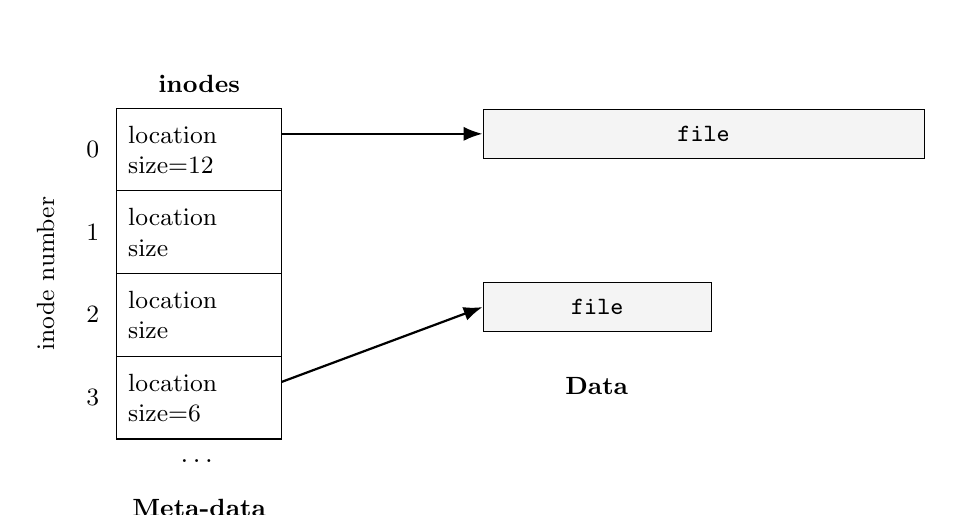
\begin{tikzpicture}
  \inodecol
  \node[dbox, minimum width=5.6cm] (b0) at (3.6,0.2) {file};
  \node[dbox, minimum width=2.9cm] (b3) at (3.6,-2.0) {file};
  \draw[locarrow] ($(i0.east)+(0,0.2)$) -- (b0.west);
  \draw[locarrow] ($(i3.east)+(0,0.2)$) -- (b3.west);
  \node[font=\small\bfseries] at (0,-4.55) {Meta-data};
  \node[font=\small\bfseries] at (5.05,-3.0) {Data};
\end{tikzpicture}
\end{center}

\begin{itemize}
  \item Inode 0 describes a file of 12 bytes (\texttt{size=12}); its data is
        the long box.
  \item Inode 3 describes a file of 6 bytes (\texttt{size=6}); its data is
        the short box.
  \item Inodes 1 and 2 are not used by any file yet (no arrow).
\end{itemize}

\keepspace{7\baselineskip}
\subsection{File API, attempt 1: name files by inode number}

If inode numbers are the names, the API is simple:

\begin{lstlisting}[numbers=none]
read(int inode, void *buf, size_t nbyte)
write(int inode, void *buf, size_t nbyte)
seek(int inode, off_t offset)
\end{lstlisting}

\textbf{\texttt{seek} does not cause a disk seek until read/write}: it only
records the position for the next read or write.

\begin{quizbox}[Disadvantages?]
\begin{itemize}
  \item Names are hard to remember.
  \item No organization or meaning to inode numbers.
  \item Semantics of offset across multiple processes? The offset would belong
        to the file, so one process's \texttt{seek} could move another's
        position (fixed by file descriptors, Section~\ref{sec:fd}).
\end{itemize}
\end{quizbox}

\keepspace{7\baselineskip}
% ===========================================================================
\section{Paths and directories}\label{sec:paths}
% ===========================================================================

\subsection{Paths}

\begin{itemize}
  \item String names are friendlier than number names.
  \item The file system still interacts with inode numbers internally.
\end{itemize}

\begin{quizbox}[Where to store \emph{path-to-inode} mappings?]
Store the \emph{path-to-inode} mappings in a predetermined \textbf{``root''
file} (typically \textbf{inode 2}). That file is a \textbf{directory}!
\end{quizbox}

\subsection{The root directory is just a file}

Start again from the inode table, but now forget what the data boxes contain
(the slides empty both boxes and drop the ``Meta-data''/``Data'' labels).
Then use the unused inode 2 as the \textbf{root directory}: its data is a list
of \texttt{"name": inode-number} pairs.

\begin{center}
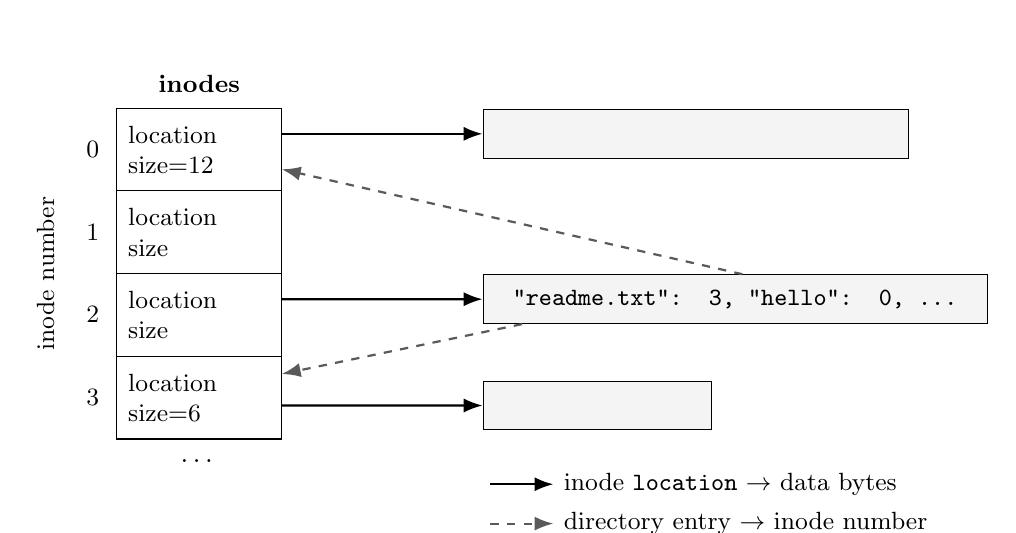
\begin{tikzpicture}
  \inodecol
  \node[dbox, minimum width=5.4cm] (b0) at (3.6,0.2) {\phantom{x}};
  \node[dbox, minimum width=6.4cm] (b2) at (3.6,-1.9) {"readme.txt": 3, "hello": 0, \ldots};
  \node[dbox, minimum width=2.9cm] (b3) at (3.6,-3.25) {\phantom{x}};
  \draw[locarrow] ($(i0.east)+(0,0.2)$) -- (b0.west);
  \draw[locarrow] ($(i2.east)+(0,0.2)$) -- (b2.west);
  \draw[locarrow] ($(i3.east)+(0,-0.1)$) -- (b3.west);
  \draw[namearrow] ($(b2.north west)+(3.3,0)$) -- ($(i0.east)+(0,-0.25)$);
  \draw[namearrow] ($(b2.south west)+(0.5,0)$) -- ($(i3.east)+(0,0.3)$);
  % legend
  \draw[locarrow] (3.7,-4.25) -- ++(0.8,0) node[right, font=\small, black] {inode \texttt{location} $\to$ data bytes};
  \draw[namearrow] (3.7,-4.75) -- ++(0.8,0) node[right, font=\small, black] {directory entry $\to$ inode number};
\end{tikzpicture}
\end{center}

\begin{itemize}
  \item Inode 2 (the root directory) points to its data, which says
        \texttt{"readme.txt"} is inode 3 and \texttt{"hello"} is inode 0.
  \item The dashed arrows (added on the next slide of the animation) show
        these name-to-inode mappings. To read
        \texttt{readme.txt}, the file system reads the root directory's data,
        finds the number 3, and then uses inode 3 to find the 6 bytes of the
        file.
\end{itemize}

\subsection{Directory tree}

\textbf{Generalize!} Use a \textbf{directory tree} instead of a single root
directory.
\begin{itemize}
  \item Only the \textbf{file name} needs to be unique \emph{within its
        directory}: \texttt{/usr/dusseau/file.txt} and
        \texttt{/tmp/file.txt} are two different files with the same name
        \texttt{file.txt}.
  \item Store a file-to-inode mapping \textbf{for each directory}.
\end{itemize}

\keepspace{7\baselineskip}
\begin{defbox}[Directory]
A directory is like a file: it also has a low-level name (an inode number).
\begin{itemize}
  \item It contains a list of \textbf{(user-readable name, low-level name)
        pairs}.
  \item Each entry in a directory refers to either \emph{files} or other
        \emph{directories}.
\end{itemize}
Example: a directory has an entry (\texttt{"foo"}, \texttt{"10"}). This means
there is a file \texttt{"foo"} with the low-level name \texttt{"10"}.
\end{defbox}

\keepspace{7\baselineskip}
\subsection{Directory tree (directory hierarchy)}

Directories can contain directories, so the names form a tree. A path is
written by listing the directories from the root, separated by
\texttt{/}.

\begin{center}
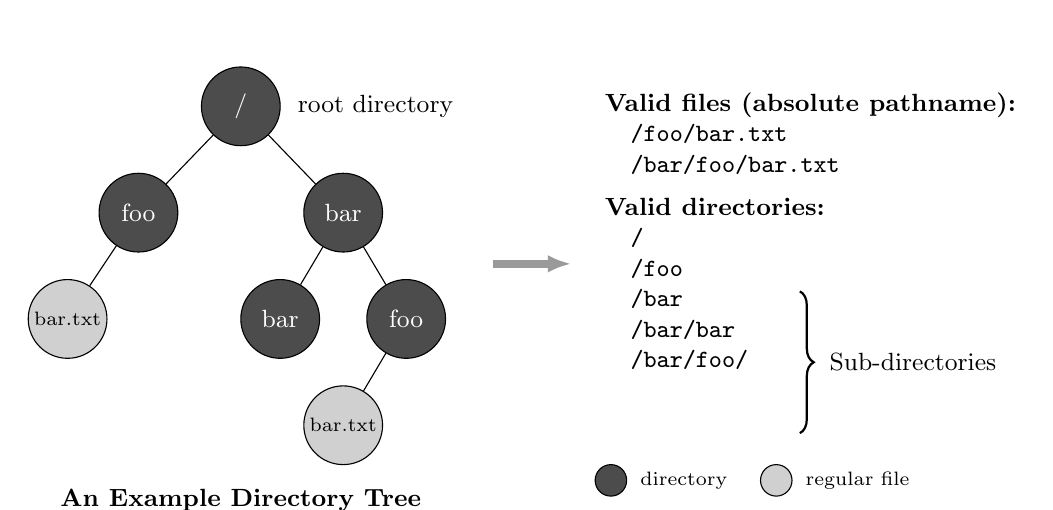
\begin{tikzpicture}[dn/.style={circle, draw, fill=black!70, text=white,
    minimum size=1.0cm, inner sep=1pt, font=\small},
    fn/.style={circle, draw, fill=g1, text=black, minimum size=1.0cm,
    inner sep=1pt, font=\scriptsize}]
  \node[dn] (r) at (2.2,0) {/};
  \node[font=\small, anchor=west] at (2.8,0) {root directory};
  \node[dn] (foo) at (0.9,-1.35) {foo};
  \node[dn] (bar) at (3.5,-1.35) {bar};
  \node[fn] (bt1) at (0,-2.7) {bar.txt};
  \node[dn] (bb) at (2.7,-2.7) {bar};
  \node[dn] (bf) at (4.3,-2.7) {foo};
  \node[fn] (bt2) at (3.5,-4.05) {bar.txt};
  \draw (r) -- (foo); \draw (r) -- (bar);
  \draw (foo) -- (bt1); \draw (bar) -- (bb); \draw (bar) -- (bf); \draw (bf) -- (bt2);
  \node[font=\small\bfseries] at (2.2,-5.0) {An Example Directory Tree};
  % arrow
  \draw[-{Latex[length=3mm]}, line width=3pt, g2] (5.4,-2.0) -- (6.4,-2.0);
  % lists
  \node[anchor=north west, align=left, font=\small] at (6.7,0.3) {%
    \textbf{Valid files (absolute pathname):}\\
    \quad\texttt{/foo/bar.txt}\\
    \quad\texttt{/bar/foo/bar.txt}\\[0.5em]
    \textbf{Valid directories:}\\
    \quad\texttt{/}\\
    \quad\texttt{/foo}\\
    \quad\texttt{/bar}\\
    \quad\texttt{/bar/bar}\\
    \quad\texttt{/bar/foo/}};
  \draw[decorate, decoration={brace, amplitude=5pt}, thick]
    (9.3,-2.35) -- (9.3,-4.15) node[midway, right=7pt, font=\small] {Sub-directories};
  % legend
  \node[dn, minimum size=0.4cm] at (6.9,-4.75) {};
  \node[font=\scriptsize, anchor=west] at (7.15,-4.75) {directory};
  \node[fn, minimum size=0.4cm] at (9.0,-4.75) {};
  \node[font=\scriptsize, anchor=west] at (9.25,-4.75) {regular file};
\end{tikzpicture}
\end{center}

\begin{itemize}
  \item The \textbf{root directory} is \texttt{/}; absolute pathnames start
        from it.
  \item The two \texttt{bar.txt} files have different full paths, so there is
        no clash.
\end{itemize}

\keepspace{7\baselineskip}
% ===========================================================================
\section{Looking up a pathname: traversal}
% ===========================================================================

Now put a small directory tree into the inode table. The root directory (inode
2) contains an entry for \texttt{etc}; the directory \texttt{etc} (inode 0)
contains an entry for \texttt{bashrc}; the file \texttt{bashrc} (inode 3)
contains some settings. The slides then animate \textbf{read
\texttt{/etc/bashrc}}, with a counter of the reads needed, from
\textbf{reads: 0} up to \textbf{reads: 6}. The numbered black circles in the
figure mark the order of the six reads.

\begin{center}
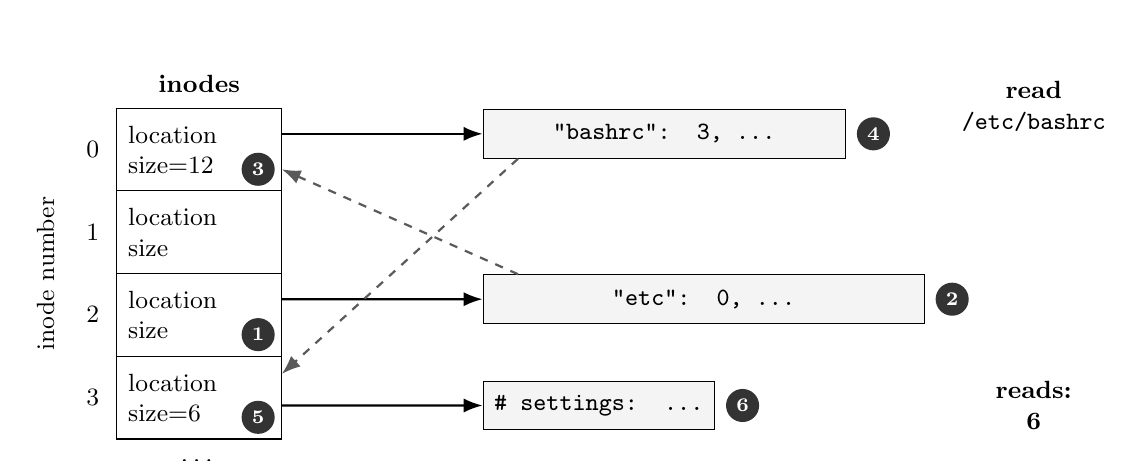
\begin{tikzpicture}
  \inodecol
  \node[dbox, minimum width=4.6cm] (b0) at (3.6,0.2) {"bashrc": 3, \ldots};
  \node[dbox, minimum width=5.6cm] (b2) at (3.6,-1.9) {"etc": 0, \ldots};
  \node[dbox, minimum width=2.9cm] (b3) at (3.6,-3.25) {\# settings: \ldots};
  \draw[locarrow] ($(i0.east)+(0,0.2)$) -- (b0.west);
  \draw[locarrow] ($(i2.east)+(0,0.2)$) -- (b2.west);
  \draw[locarrow] ($(i3.east)+(0,-0.1)$) -- (b3.west);
  \draw[namearrow] ($(b2.north west)+(0.45,0)$) -- ($(i0.east)+(0,-0.25)$);
  \draw[namearrow] ($(b0.south west)+(0.45,0)$) -- ($(i3.east)+(0,0.3)$);
  % read order
  \node[badge] at ($(i2.east)+(-0.3,-0.25)$) {1};
  \node[badge] at ($(b2.east)+(0.35,0)$) {2};
  \node[badge] at ($(i0.east)+(-0.3,-0.25)$) {3};
  \node[badge] at ($(b0.east)+(0.35,0)$) {4};
  \node[badge] at ($(i3.east)+(-0.3,-0.25)$) {5};
  \node[badge] at ($(b3.east)+(0.35,0)$) {6};
  \node[font=\small\bfseries, align=center] at (10.6,0.55) {read\\\texttt{/etc/bashrc}};
  \node[font=\small\bfseries, align=center] at (10.6,-3.25) {reads:\\6};
\end{tikzpicture}
\end{center}

{\small (On the slides the root directory's entry for the file reads
\texttt{"bashrc": 6}, but the dashed arrow and the highlighted inode in the
animation are inode 3, the only file inode in the table. The entry should say
\texttt{"bashrc": 3}, which is what is drawn here.)}

\begin{center}
\small
\renewcommand{\arraystretch}{1.2}
\begin{tabularx}{\textwidth}{@{}clX@{}}
  \toprule
  \textbf{reads} & \textbf{What is read} & \textbf{What it tells us} \\
  \midrule
  0 & (nothing yet) & start of the lookup of \texttt{/etc/bashrc} \\
  1 & inode 2 (root directory's inode) & where the root directory's data is
      (inode 2 is known in advance) \\
  2 & root directory's data, \texttt{"etc": 0, \ldots} & \texttt{etc} is
      inode 0 \\
  3 & inode 0 (\texttt{etc} directory's inode) & where the \texttt{etc}
      directory's data is \\
  4 & \texttt{etc}'s data, \texttt{"bashrc": 3, \ldots} & \texttt{bashrc} is
      inode 3 \\
  5 & inode 3 (\texttt{bashrc}'s inode) & where the file's bytes are, and its
      size (6) \\
  6 & \texttt{bashrc}'s data, \texttt{\# settings: \ldots} & the bytes the
      program asked for \\
  \bottomrule
\end{tabularx}
\end{center}

\begin{keybox}[Traversal]
To read \texttt{/etc/bashrc}: read the root dir (inode and data); read the
\texttt{etc} dir (inode and data); read the \texttt{bashrc} file (inode and
data). {\small (The slide misspells ``inode'' as ``indode''.)}

The reads for getting to the final inode are called the \textbf{traversal}.
\end{keybox}

% ===========================================================================
\section{Directory calls and special entries}
% ===========================================================================

\subsection{Directory calls}

\begin{itemize}
  \item \texttt{mkdir}: create a new directory.
  \item \texttt{readdir}: read/parse directory entries.
\end{itemize}
Both are covered in more detail in Section~\ref{sec:dirs}.

\begin{quizbox}[Why no \texttt{writedir}?]
Directory contents are file-system metadata that must stay well formed, so
programs cannot write a directory directly; they change it only indirectly
(creating, renaming, linking or deleting files inside it).
\end{quizbox}

\keepspace{7\baselineskip}
\subsection{Special directory entries: \texttt{.} and \texttt{..}}

\begin{center}
\small\ttfamily
\begin{tabular}{@{}l@{}}
\$ ls -la\\
total 728\\
drwxr-xr-x\ \ 34 trh\ staff\ \ 1156 Oct 19 11:41 \textbf{.}\\
drwxr-xr-x+ 59 trh\ staff\ \ 2006 Oct\ \ 8 15:49 \textbf{..}\\
\strike{-rw-r--r--@\ \ 1 trh\ staff\ \ 6148 Oct 19 11:42 .DS\_Store}\\
\strike{-rw-r--r--\ \ \ 1 trh\ staff\ \ \ 553 Oct\ \ 2 14:29 asdf.txt}\\
\strike{-rw-r--r--\ \ \ 1 trh\ staff\ \ \ 553 Oct\ \ 2 14:05 asdf.txt\textasciitilde}\\
drwxr-xr-x\ \ \ 4 trh\ staff\ \ \ 136 Jun 18 15:37 backup\\
\ldots
\end{tabular}
\end{center}
\keepspace{0pt}

The slide strikes out the ordinary files to focus on the first two lines.
Every directory contains two special entries:
\begin{itemize}
  \item \textbf{\texttt{.}} (``dot'') is an entry for \textbf{the directory
        itself};
  \item \textbf{\texttt{..}} (``dot-dot'') is an entry for its
        \textbf{parent directory}.
\end{itemize}
\textbf{Try it:} \texttt{cd /; ls -lia} (\texttt{-i} shows inode numbers).
In the root directory, \texttt{.} and \texttt{..} have the same inode
number, because the root has no parent.

\keepspace{7\baselineskip}
% ===========================================================================
\section{File descriptors}\label{sec:fd}
% ===========================================================================

\subsection{File API, attempt 2: name files by path}

\begin{lstlisting}[numbers=none]
read(char *path, void *buf, size_t nbyte)
write(char *path, void *buf, size_t nbyte)
\end{lstlisting}

\begin{quizbox}[Disadvantages?]
\textbf{Expensive traversal!} Every \texttt{read} or \texttt{write} would
repeat the whole path lookup.

\textbf{Goal: traverse once.}
\end{quizbox}

Three types of names: inode, path, \textbf{file descriptor}.

\subsection{The file descriptor idea}

\begin{defbox}[File descriptor (fd)]
\textbf{Idea:}
\begin{itemize}
  \item Do the expensive traversal \textbf{once} (when the file is
        \emph{opened}), and store the inode in a \textbf{descriptor object}
        (kept in memory).
  \item Do reads/writes via the descriptor, which also \textbf{tracks the
        offset}.
\end{itemize}
\textbf{Each process} has a \textbf{file-descriptor table} that contains
pointers to open-file entries (\texttt{struct file} / open file table
entries). The integers used for file I/O are the descriptors: they are
\textbf{indexes into this table}. By convention
\texttt{stdin} is 0, \texttt{stdout} is 1 and \texttt{stderr} is 2.
\end{defbox}

\keepspace{7\baselineskip}
\subsection{FD table in xv6}


\begin{lstlisting}
struct file {
  ...
  struct inode *ip;
  uint off;
};

// Per-process state
struct proc {
  ...
  struct file *ofile[NOFILE];  // Open files
  ...
};
\end{lstlisting}
{\small (The slide closes \texttt{struct proc} with \texttt{\char`\}} and no
semicolon; it is added here.)}

\texttt{struct file} is one open file (inode pointer + offset);
\texttt{ofile} is the process's fd table, and an fd is an index into it.

\keepspace{7\baselineskip}
\subsection{Code snippet, step by step}

\begin{lstlisting}
int fd1 = open("file.txt"); // returns 3
read(fd1, buf, 12);
int fd2 = open("file.txt"); // returns 4
int fd3 = dup(fd2);         // returns 5
\end{lstlisting}

\texttt{open} returns the lowest unused slot (0, 1, 2 are stdin, stdout,
stderr). \texttt{dup(fd)} makes a new fd for the \textbf{same} open file.
The slides animate the snippet one line at a time:

\keepspace{7\baselineskip}
\begin{center}
\begin{minipage}{\textwidth}
\begin{minipage}[t]{0.49\textwidth}\centering
\fdpic{0}{
  \node[font=\scriptsize, align=center, below=2pt] at (I.south) {``file.txt'' also\\points here};}\\[0.3em]
{\small (1) \texttt{int fd1 = open("file.txt");} \(\to\) 3}
\end{minipage}\hfill
\begin{minipage}[t]{0.49\textwidth}\centering
\fdpic{12}{}\\[0.3em]
{\small (2) \texttt{read(fd1, buf, 12);}}
\end{minipage}
\end{minipage}
\end{center}
\keepspace{7\baselineskip}
\begin{center}
\begin{minipage}{\textwidth}
\begin{minipage}[t]{0.49\textwidth}\centering
\fdpic{12}{\fdB}\\[0.3em]
{\small (3) \texttt{int fd2 = open("file.txt");} \(\to\) 4}
\end{minipage}\hfill
\begin{minipage}[t]{0.49\textwidth}\centering
\fdpic{12}{\fdB
  \draw[->, thick] (f5.center) -- ($(B.west)+(0,-0.15)$);}\\[0.3em]
{\small (4) \texttt{int fd3 = dup(fd2);} \(\to\) 5}
\end{minipage}
\end{minipage}
\end{center}

\begin{enumerate}
  \item \texttt{open} returns 3: one traversal; a new open file with
        \texttt{offset = 0} points to the inode (which \texttt{"file.txt"}
        also points to).
  \item \texttt{read(fd1, buf, 12)}: no lookup; the offset becomes 12.
  \item The second \texttt{open} returns 4: a \textbf{new} open file with its
        own \texttt{offset = 0}, same inode.
  \item \texttt{dup(fd2)} returns 5: slot 5 points to the \textbf{same} open
        file as slot 4, so fds 4 and 5 share one offset.
\end{enumerate}

\keepspace{7\baselineskip}
\subsection{File API, attempt 3: open, then use the descriptor}

\begin{lstlisting}[numbers=none]
int fd = open(char *path, int flag, mode_t mode)
read(int fd, void *buf, size_t nbyte)
write(int fd, void *buf, size_t nbyte)
close(int fd)
\end{lstlisting}

\keepspace{7\baselineskip}
\begin{keybox}[Advantages]
\begin{itemize}
  \item \textbf{string names} (paths are easy to remember);
  \item \textbf{hierarchical} (directories organize files);
  \item \textbf{traverse once} (only in \texttt{open});
  \item \textbf{different offsets precisely defined} (each \texttt{open} has
        its own offset; \texttt{dup} shares one).
\end{itemize}
\end{keybox}

% ===========================================================================
\section{Reading and writing files}
% ===========================================================================

\subsection{An example: \texttt{echo} and \texttt{cat}}

An example of reading and writing a file \texttt{foo}:
\begin{itemize}
  \item \texttt{echo hello > foo}: redirect the output of \texttt{echo} to
        the file \texttt{foo};
  \item \texttt{cat foo}: dump the contents of a file to the screen.
\end{itemize}

\begin{lstlisting}[style=term]
prompt> echo hello > foo
prompt> cat foo
hello
prompt>
\end{lstlisting}

\begin{quizbox}[How does the \texttt{cat} program access the file \texttt{foo}?]
We can use \textbf{\texttt{strace}} to trace the system calls made by a
program.
\end{quizbox}

\keepspace{7\baselineskip}
\begin{lstlisting}[style=term]
prompt> strace cat foo
...
open("foo", O_RDONLY|O_LARGEFILE)   = 3
read(3, "hello\n", 4096)            = 6
write(1, "hello\n", 6)              = 6   // file descriptor 1: standard out
hello
read(3, "", 4096)                   = 0   // 0: no bytes left in the file
close(3)                            = 0
...
prompt>
\end{lstlisting}

\texttt{cat} opens \texttt{foo} read-only (fd 3), reads 6 bytes, writes them
to fd 1 (the screen), reads again and gets 0 (end of file), and closes fd 3.

\begin{keybox}[The calls]
\begin{itemize}
  \item \texttt{open(pathname, flags)}: returns a file descriptor (3 in the
        example). File descriptors 0, 1, 2 are for standard input, output and
        error. {\small (The slide writes \texttt{open(file descriptor,
        flags)}; \texttt{open} takes a path, and returns the descriptor.)}
  \item \texttt{read(file descriptor, buffer pointer, size of the buffer)}:
        returns the number of bytes it read.
  \item \texttt{write(file descriptor, buffer pointer, size of the buffer)}:
        returns the number of bytes it wrote. {\small (The slide says ``it write''.)}
\end{itemize}
\end{keybox}

\textbf{Writing a file} takes a similar set of steps:
\begin{enumerate}
  \item the file is opened for writing (\texttt{open()});
  \item the \texttt{write()} system call is called, repeatedly for larger
        files;
  \item \texttt{close()}.
\end{enumerate}

\keepspace{7\baselineskip}
\subsection{Reading and writing, but not sequentially}

An open file has a \textbf{current offset}. It determines \textbf{where} the
next read or write will begin reading from or writing to within the file.
The current offset is updated in two ways:
\begin{itemize}
  \item \textbf{Implicitly:} a read or write of \(N\) bytes adds \(N\) to
        the current offset.
  \item \textbf{Explicitly:} with \texttt{lseek()}.
\end{itemize}

\begin{lstlisting}[numbers=none]
off_t lseek(int fildes, off_t offset, int whence);
\end{lstlisting}
\begin{itemize}
  \item \texttt{fildes}: the file descriptor;
  \item \texttt{offset}: positions the file offset to a particular location
        within the file;
  \item \texttt{whence}: determines how the seek is performed.
\end{itemize}

From the man page:
\begin{lstlisting}[style=term]
If whence is SEEK_SET, the offset is set to offset bytes.
If whence is SEEK_CUR, the offset is set to its current location plus offset bytes.
If whence is SEEK_END, the offset is set to the size of the file plus offset bytes.
\end{lstlisting}

(\texttt{lseek} only changes the offset in memory; it does no disk I/O.)

\keepspace{7\baselineskip}
% ===========================================================================
\section{Writing immediately with \texttt{fsync()}}
% ===========================================================================

\begin{itemize}
  \item The file system will \textbf{buffer} writes in memory for some time,
        e.g.\ 5 seconds, or 30, for \textbf{performance} reasons.
  \item At that later point in time, the write(s) will \textbf{actually be
        issued} to the storage device.
  \begin{itemize}
    \item Writes seem to \textbf{complete quickly}.
    \item Data can be \textbf{lost} (e.g., the machine crashes).
  \end{itemize}
\end{itemize}

However, some applications require more than this \emph{eventual}
guarantee. Example: a DBMS requires force writes to disk from time to time.

\begin{lstlisting}[numbers=none]
int fsync(int fd)
\end{lstlisting}
{\small (The slide shows the return type as \texttt{off\_t}; \texttt{fsync}
returns \texttt{int}: 0 on success, \(-1\) on error.)}
\begin{itemize}
  \item The file system forces the file's \textbf{dirty} (i.e., not yet written)
        data \textbf{and} its metadata (inode, size) to disk for the file
        referred to by the file descriptor. {\small (The slide says ``file description''.)}
  \item \texttt{fsync()} returns once all of these writes are complete.
\end{itemize}

\keepspace{7\baselineskip}
\subsection{An example of \texttt{fsync()}}

\begin{lstlisting}
int fd = open("foo", O_CREAT | O_WRONLY | O_TRUNC);
assert (fd > -1);
int rc = write(fd, buffer, size);
assert (rc == size);
rc = fsync(fd);
assert (rc == 0);
\end{lstlisting}
{\small (The slide has no semicolon after \texttt{assert (fd > -1)}.)}
{\small (In real code, \texttt{open} with \texttt{O\_CREAT} also takes a third
\texttt{mode} argument, e.g.\ \texttt{0644} or \texttt{S\_IRUSR|S\_IWUSR};
the slides omit it.)}

\begin{warnbox}[In some cases, also \texttt{fsync()} the directory]
In some cases, this code also needs to \texttt{fsync()} the
\textbf{directory} that contains \texttt{foo}: if \texttt{foo} was just
created, its name is in the directory's data, which \texttt{fsync(fd)} does
not flush.
\end{warnbox}

\keepspace{7\baselineskip}
% ===========================================================================
\section{Renaming files: \texttt{rename()}}
% ===========================================================================

\begin{lstlisting}[numbers=none]
rename(char *old, char *new)
\end{lstlisting}
\begin{itemize}
  \item Renames a file to a different name.
  \item It is implemented as an \textbf{atomic call} (after a crash the file
        has either the old name or the new name).
\end{itemize}

\textbf{Example: change from \texttt{foo} to \texttt{bar}.}
\begin{lstlisting}[style=term]
prompt> mv foo bar      // mv uses the system call rename()
\end{lstlisting}

\textbf{Example: how to update a file atomically.}
\begin{lstlisting}
int fd = open("foo.txt.tmp", O_WRONLY|O_CREAT|O_TRUNC);
write(fd, buffer, size); // write out new version of file
fsync(fd);
close(fd);
rename("foo.txt.tmp", "foo.txt");
\end{lstlisting}
{\small (The slide's first line reads \texttt{int fint fd = \ldots}; the stray
\texttt{fint} is a typo.)}

Write the new version to a temporary file, \texttt{fsync} it, then
\texttt{rename} it over the old name: after a crash, \texttt{foo.txt} is
either the complete old version or the complete new one.

\keepspace{7\baselineskip}
% ===========================================================================
\section{Getting information about files: \texttt{stat()}}
% ===========================================================================

\texttt{stat()}, \texttt{fstat()}: show the file \textbf{metadata}.
\begin{itemize}
  \item \textbf{Metadata} is information about each file, e.g.\ size,
        low-level name (inode number), permissions, \ldots
\end{itemize}

\begin{lstlisting}
struct stat {
  dev_t     st_dev;     /* ID of device containing file */
  ino_t     st_ino;     /* inode number */
  mode_t    st_mode;    /* protection */
  nlink_t   st_nlink;   /* number of hard links */
  uid_t     st_uid;     /* user ID of owner */
  gid_t     st_gid;     /* group ID of owner */
  dev_t     st_rdev;    /* device ID (if special file) */
  off_t     st_size;    /* total size, in bytes */
  blksize_t st_blksize; /* blocksize for filesystem I/O */
  blkcnt_t  st_blocks;  /* number of blocks allocated */
  time_t    st_atime;   /* time of last access */
  time_t    st_mtime;   /* time of last modification */
  time_t    st_ctime;   /* time of last status change */
};
\end{lstlisting}

\keepspace{7\baselineskip}
To see stat information, you can use the command-line tool \texttt{stat}:

\begin{lstlisting}[style=term]
prompt> echo hello > file
prompt> stat file
  File: 'file'
  Size: 6           Blocks: 8          IO Block: 4096   regular file
Device: 811h/2065d  Inode: 67158084    Links: 1
Access: (0640/-rw-r-----)  Uid: (30686/ root)   Gid: (30686/ remzi)
Access: 2011-05-03 15:50:20.157594748 -0500
Modify: 2011-05-03 15:50:20.157594748 -0500
Change: 2011-05-03 15:50:20.157594748 -0500
\end{lstlisting}

\keepspace{7\baselineskip}
The file system keeps this type of information in the \textbf{inode}.

\keepspace{7\baselineskip}
% ===========================================================================
\section{Removing files: \texttt{unlink()}}
% ===========================================================================

\texttt{rm} is the Linux command to remove a file. \texttt{rm} calls
\texttt{unlink()} to remove a file:

\begin{lstlisting}[style=term]
prompt> strace rm foo
...
unlink("foo")        = 0   // return 0 upon success
...
prompt>
\end{lstlisting}

\begin{quizbox}[Why does it call \texttt{unlink()}, not ``remove'' or ``delete''?]
``We can get the answer later'' (Section~\ref{sec:hard}): \texttt{unlink}
removes one \emph{name} (link) to the inode; the file is freed only when the
last name is gone.
\end{quizbox}

\keepspace{7\baselineskip}
% ===========================================================================
\section{Directories: \texttt{mkdir}, \texttt{readdir}, \texttt{rmdir}}\label{sec:dirs}
% ===========================================================================

\subsection{Making directories: \texttt{mkdir()}}

\begin{lstlisting}[style=term]
prompt> strace mkdir foo
...
mkdir("foo", 0777)   = 0
prompt>
\end{lstlisting}

(\texttt{0777} is the requested permission; 0 means success.)

\begin{itemize}
  \item When a directory is created, it is \textbf{empty}.
  \item An empty directory has two entries: \texttt{.} (itself) and
        \texttt{..} (its parent).
\end{itemize}

\begin{lstlisting}[style=term]
prompt> ls -a
./  ../
prompt> ls -al
total 8
drwxr-x---  2 minati minati    6 Apr 30 16:17 ./
drwxr-x--- 26 minati minati 4096 Apr 30 16:17 ../
\end{lstlisting}
{\small (The slide types the first option with an en-dash instead of a
hyphen; the flag is \texttt{-a}.)}

\keepspace{18\baselineskip}
\subsection{Reading directories: \texttt{opendir}, \texttt{readdir}, \texttt{closedir}}

A sample program that reads directory entries (like \texttt{ls}):

\begin{lstlisting}
int main(int argc, char *argv[]) {
  DIR *dp = opendir(".");             // open current directory
  assert(dp != NULL);
  struct dirent *d;
  while ((d = readdir(dp)) != NULL)   // read one directory entry
  {
    // print out the name and inode number of each file
    printf("%d %s\n", (int) d->d_ino, d->d_name);
  }
  closedir(dp);                       // close current directory
  return 0;
}
\end{lstlisting}

Each \texttt{readdir} returns the next entry (\texttt{NULL} at the end).
The information available within \texttt{struct dirent}:

\begin{lstlisting}
struct dirent {
  char           d_name[256]; /* filename */
  ino_t          d_ino;       /* inode number */
  off_t          d_off;       /* offset to the next dirent */
  unsigned short d_reclen;    /* length of this record */
  unsigned char  d_type;      /* type of file */
};
\end{lstlisting}
{\small (On the slide the \texttt{d\_off} comment is cut off as ``offset to
the next direct'', and the closing \texttt{\char`\}} has no semicolon.)}

\subsection{Deleting directories: \texttt{rmdir()}}

\begin{itemize}
  \item \texttt{rmdir()} deletes a directory.
  \item It requires that the directory be \textbf{empty}, i.e., it only has
        the \texttt{"."} and \texttt{".."} entries.
  \item If you call \texttt{rmdir()} on a non-empty directory, it will fail.
\end{itemize}

\keepspace{7\baselineskip}
% ===========================================================================
\section{Hard links}\label{sec:hard}
% ===========================================================================

\begin{lstlisting}[numbers=none]
link(old pathname, new one)
\end{lstlisting}
{\small (``new one'' means the new pathname.)}
\begin{itemize}
  \item \textbf{Links} a new file name to an old one.
  \item Creates another way to refer to \emph{the same file}.
  \item The command-line link program is \texttt{ln}.
\end{itemize}

\begin{lstlisting}[style=term]
prompt> echo hello > file
prompt> cat file
hello
prompt> ln file file2     // create a hard link, link file to file2
prompt> cat file2
hello
\end{lstlisting}

\begin{defbox}[How \texttt{link} works]
\begin{itemize}
  \item \textbf{Create} another name in the directory.
  \item \textbf{Refer} it to the \textbf{same inode number} of the original
        file. The file is \textbf{not copied} in any way.
  \item Then we just have two human names (\texttt{file} and
        \texttt{file2}) that both refer to the same file.
\end{itemize}
\end{defbox}

\keepspace{7\baselineskip}
\textbf{The result of \texttt{link()}:} the two files have the \textbf{same
inode number}, but two human names (\texttt{file}, \texttt{file2}).

\begin{lstlisting}[style=term]
prompt> ls -i
67158084 file      /* inode value is 67158084 */
67158084 file2     /* inode value is 67158084 */
prompt>
\end{lstlisting}

There is \textbf{no difference} between \texttt{file} and \texttt{file2}:
both are just links to the underlying metadata about the file.

\keepspace{7\baselineskip}
\subsection{Removing a name: \texttt{unlink()} and the reference count}

Thus, to remove a file, we call \texttt{unlink()}:

\begin{lstlisting}[style=term]
prompt> rm file
removed 'file'
prompt> cat file2         // Still access the file
hello
\end{lstlisting}

\keepspace{7\baselineskip}
\begin{defbox}[Reference count (link count)]
\begin{itemize}
  \item The \textbf{reference count} tracks how many different file names
        have been linked to this inode.
  \item When \texttt{unlink()} is called, the reference count
        \textbf{decrements}.
  \item If the reference count reaches \textbf{zero}, the file system
        \textbf{frees the inode and related data blocks}, and thus truly
        ``deletes'' the file.
\end{itemize}
\end{defbox}

\keepspace{22\baselineskip}
\subsection{Watching the link count}

\texttt{stat()} shows the reference count of a file.

\begin{lstlisting}[style=term]
prompt> echo hello > file             /* create file */
prompt> stat file
... Inode: 67158084 Links: 1 ...      /* Link count is 1 */
prompt> ln file file2                 /* hard link file2 */
prompt> stat file
... Inode: 67158084 Links: 2 ...      /* Link count is 2 */
prompt> stat file2
... Inode: 67158084 Links: 2 ...      /* Link count is 2 */
prompt> ln file2 file3                /* hard link file3 */
prompt> stat file
... Inode: 67158084 Links: 3 ...      /* Link count is 3 */
prompt> rm file                       /* remove file */
prompt> stat file2
... Inode: 67158084 Links: 2 ...      /* Link count is 2 */
prompt> rm file2                      /* remove file2 */
prompt> stat file3
... Inode: 67158084 Links: 1 ...      /* Link count is 1 */
prompt> rm file3
\end{lstlisting}

\keepspace{12\baselineskip}
The directory and the inode after each step:

\begin{center}
\hlpanel{file}{1}{(1) \texttt{echo hello > file}}\hfill
\hlpanel{file,file2}{2}{(2) \texttt{ln file file2}}\hfill
\hlpanel{file,file2,file3}{3}{(3) \texttt{ln file2 file3}}

\medskip
\hlpanel{file2,file3}{2}{(4) \texttt{rm file}}\hfill
\hlpanel{file3}{1}{(5) \texttt{rm file2}}\hfill
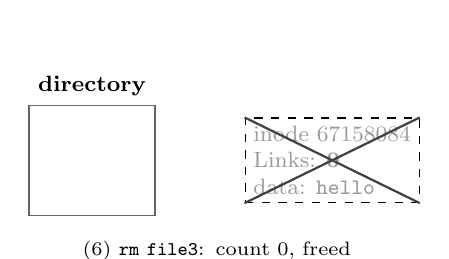
\begin{tikzpicture}[font=\footnotesize]
  \node[font=\footnotesize\bfseries] at (0,0.05) {directory};
  \draw[boxline] (-0.8,-0.2) rectangle (0.8,-1.6);
  \node[draw, dashed, text=g2, align=left, inner sep=3pt, font=\footnotesize] (I) at (3.05,-0.9)
    {inode 67158084\\Links: \textbf{0}\\data: \texttt{hello}};
  \draw[black!75, line width=0.8pt] (I.south west) -- (I.north east);
  \draw[black!75, line width=0.8pt] (I.north west) -- (I.south east);
  \node[font=\scriptsize, text width=4.6cm, align=center] at (1.6,-2.05) {(6) \texttt{rm file3}: count 0, freed};
\end{tikzpicture}
\end{center}
\keepspace{0pt}



\keepspace{7\baselineskip}
% ===========================================================================
\section{Symbolic links (soft links)}
% ===========================================================================

A \textbf{symbolic link} is more \textbf{useful} than a hard link, because
hard links have two limits:
\begin{itemize}
  \item \textbf{A hard link cannot be created to a directory}, for fear that
        you will create a \textbf{cycle} in the directory tree.
  \item \textbf{A hard link cannot be created to a file in another
        partition}, because inode numbers are only unique within a file
        system.
\end{itemize}

Create a symbolic link with \texttt{ln -s}:
\begin{lstlisting}[style=term]
prompt> echo hello > file
prompt> ln -s file file2    /* option -s : create a symbolic link */
prompt> cat file2
hello
\end{lstlisting}
{\small (The slide types the option with an en-dash instead of a hyphen,
and ends the comment with a stray comma; the option is \texttt{-s}.)}

\keepspace{7\baselineskip}
\begin{quizbox}[What is the difference between a symbolic link and a hard link?]
\begin{itemize}
  \item A symbolic link is \textbf{a file itself}, of a different type:
        symbolic links are \textbf{a third type} the file system knows about
        (besides regular files and directories). It has its own inode.
  \item The size of the symbolic link \texttt{file2} is \textbf{4 bytes}: a
        symbolic link holds the \textbf{pathname} of the linked-to file as
        the data of the link file, and \texttt{"file"} is 4 characters.
  \item A hard link is only a directory entry with the same inode number; a
        symbolic link stores a \emph{name} and is resolved by looking that
        name up again each time it is used.
\end{itemize}
\end{quizbox}

\begin{lstlisting}[style=term]
prompt> stat file
 ... regular file ...
prompt> stat file2
 ... symbolic link ...    // Actually a file itself of a different type
\end{lstlisting}

\begin{lstlisting}[style=term]
prompt> ls -al
drwxr-x---  2 remzi remzi   29 May 3 19:10 ./
drwxr-x--- 27 remzi remzi 4096 May 3 15:14 ../           // directory
-rw-r-----  1 remzi remzi    6 May 3 19:10 file          // regular file
lrwxrwxrwx  1 remzi remzi    4 May 3 19:10 file2 -> file // symbolic link
\end{lstlisting}

The type letter \texttt{l} marks a symbolic link; \texttt{file2} has size
\textbf{4}.

\keepspace{7\baselineskip}
If we link to a longer pathname, our link file would be bigger:
\begin{lstlisting}[style=term]
prompt> echo hello > alongerfilename
prompt> ln -s alongerfilename file3
prompt> ls -al alongerfilename file3
-rw-r----- 1 remzi remzi  6 May 3 19:17 alongerfilename
lrwxrwxrwx 1 remzi remzi 15 May 3 19:17 file3 -> alongerfilename
\end{lstlisting}
The link \texttt{file3} has size \textbf{15}, the length of
\texttt{alongerfilename}.

\keepspace{7\baselineskip}
\subsection{Dangling reference}

When the original file is removed, the symbolic link \textbf{points to
nothing}: a \textbf{dangling reference}. {\small (The slide says ``points
noting''.)}

\begin{lstlisting}[style=term]
prompt> echo hello > file
prompt> ln -s file file2
prompt> cat file2
hello
prompt> rm file           // remove the original file
prompt> cat file2
cat: file2: No such file or directory
\end{lstlisting}

\keepspace{7\baselineskip}
\begin{center}
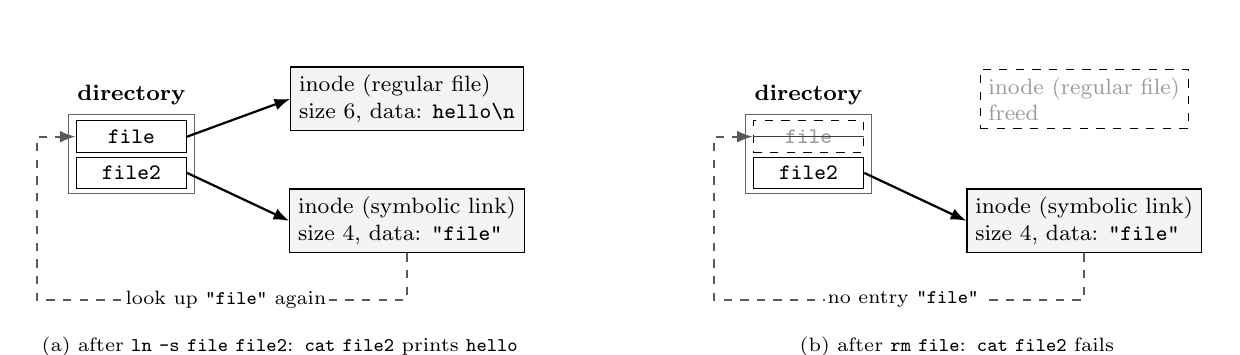
\begin{tikzpicture}[font=\footnotesize, >={Latex[length=2mm]},
    ent/.style={draw, fill=white, minimum width=1.4cm, minimum height=0.4cm,
      inner sep=1pt, font=\footnotesize\ttfamily},
    ino/.style={draw, fill=boxfill, align=left, inner sep=3pt, font=\footnotesize}]
  % before
  \begin{scope}
    \node[font=\footnotesize\bfseries] at (0,0.05) {directory};
    \draw[boxline] (-0.8,-0.2) rectangle (0.8,-1.2);
    \node[ent] (a) at (0,-0.48) {file};
    \node[ent] (b) at (0,-0.94) {file2};
    \node[ino] (A) at (3.5,0.0) {inode (regular file)\\size 6, data: \texttt{hello\char`\\n}};
    \node[ino] (B) at (3.5,-1.55) {inode (symbolic link)\\size 4, data: \texttt{"file"}};
    \draw[->, thick] (a.east) -- (A.west);
    \draw[->, thick] (b.east) -- (B.west);
    \draw[->, thick, dashed, g3] (B.south) |- (-1.2,-2.55) |- (a.west);
    \node[font=\scriptsize, fill=white, inner sep=1pt] at (1.2,-2.55) {look up \texttt{"file"} again};
    \node[font=\scriptsize, text width=6.2cm, align=center] at (1.9,-3.15) {(a) after \texttt{ln~-s file file2}: \texttt{cat file2} prints \texttt{hello}};
  \end{scope}
  % after
  \begin{scope}[xshift=8.6cm]
    \node[font=\footnotesize\bfseries] at (0,0.05) {directory};
    \draw[boxline] (-0.8,-0.2) rectangle (0.8,-1.2);
    \node[ent, text=g2, dashed] (a) at (0,-0.48) {file};
    \draw[black!75] (a.west) -- (a.east);
    \node[ent] (b) at (0,-0.94) {file2};
    \node[draw, dashed, text=g2, align=left, inner sep=3pt, font=\footnotesize] (A) at (3.5,0.0) {inode (regular file)\\freed};
    \node[ino] (B) at (3.5,-1.55) {inode (symbolic link)\\size 4, data: \texttt{"file"}};
    \draw[->, thick] (b.east) -- (B.west);
    \draw[->, thick, dashed, g3] (B.south) |- (-1.2,-2.55) |- (a.west);
    \node[font=\scriptsize, fill=white, inner sep=1pt] at (1.2,-2.55) {no entry \texttt{"file"}};
    \node[font=\scriptsize, text width=6.2cm, align=center] at (1.9,-3.15) {(b) after \texttt{rm file}: \texttt{cat file2} fails};
  \end{scope}
\end{tikzpicture}
\end{center}

The symbolic link still exists, but the name it holds no longer leads
anywhere (unlike a hard link, where \texttt{cat file2} kept working).

\keepspace{7\baselineskip}
% ===========================================================================
\section{Many file systems: mounting}
% ===========================================================================

Users often want to use \textbf{many file systems}, for example:
\begin{itemize}
  \item the main disk,
  \item a backup disk,
  \item AFS (the Andrew File System, a network file system),
  \item thumb drives.
\end{itemize}

\begin{quizbox}[What is the most elegant way to support this?]
Approach 2 below: \textbf{mount} all file systems into \textbf{one}
directory tree.
\end{quizbox}

\keepspace{7\baselineskip}
\subsection{Approach 1: one tree per device (drive letters)}

The slide shows the Windows~7 ``Computer'' window: every file system is a
separate drive with its own letter, and every path starts with a drive
letter (e.g.\ \texttt{E:\char`\\photos}). Redrawn schematically:

\begin{center}
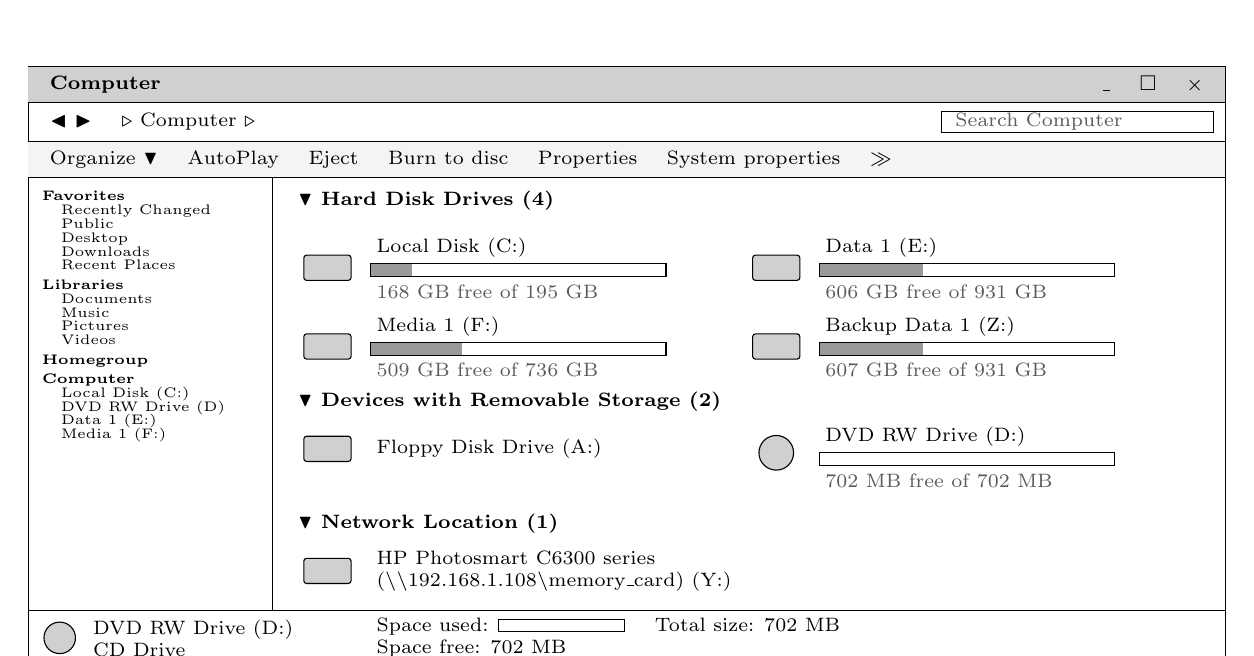
\begin{tikzpicture}[font=\scriptsize,
    drv/.style={draw, fill=g1, rounded corners=1pt, minimum width=0.6cm, minimum height=0.32cm, inner sep=0pt}]
  \draw[fill=white] (0,0) rectangle (15.2,-7.6);
  % title bar
  \fill[g1] (0,0) rectangle (15.2,-0.45);
  \node[anchor=west, font=\scriptsize\bfseries] at (0.15,-0.225) {Computer};
  \node[anchor=east] at (15.05,-0.225) {\_ \quad $\square$ \quad $\times$};
  % address bar
  \draw (0,-0.45) -- (15.2,-0.45);
  \node[anchor=west] at (0.15,-0.7) {$\blacktriangleleft$ $\blacktriangleright$ \quad $\triangleright$ Computer $\triangleright$};
  \draw (11.6,-0.57) rectangle (15.05,-0.83);
  \node[anchor=west, text=g3] at (11.65,-0.7) {Search Computer};
  % toolbar
  \fill[boxfill] (0,-0.95) rectangle (15.2,-1.4);
  \draw (0,-0.95) -- (15.2,-0.95) (0,-1.4) -- (15.2,-1.4);
  \node[anchor=west] at (0.15,-1.175) {Organize $\blacktriangledown$ \quad AutoPlay \quad Eject \quad Burn to disc \quad Properties \quad System properties \quad $\gg$};
  % left pane
  \draw (3.1,-1.4) -- (3.1,-6.9);
  \node[anchor=north west, align=left, font=\tiny, inner sep=2pt] at (0.1,-1.5) {%
    \textbf{Favorites}\\[-1pt] \quad Recently Changed\\[-1pt] \quad Public\\[-1pt] \quad Desktop\\[-1pt] \quad Downloads\\[-1pt] \quad Recent Places\\[1pt]
    \textbf{Libraries}\\[-1pt] \quad Documents\\[-1pt] \quad Music\\[-1pt] \quad Pictures\\[-1pt] \quad Videos\\[1pt]
    \textbf{Homegroup}\\[1pt]
    \textbf{Computer}\\[-1pt] \quad Local Disk (C:)\\[-1pt] \quad DVD RW Drive (D)\\[-1pt] \quad Data 1 (E:)\\[-1pt] \quad Media 1 (F:)};
  % main pane
  \node[anchor=west, font=\scriptsize\bfseries] at (3.3,-1.7) {$\blacktriangledown$ Hard Disk Drives (4)};
  \foreach \x/\y/\l/\s/\f in {3.5/-2.3/Local Disk (C:)/168 GB free of 195 GB/0.14,
                              9.2/-2.3/Data 1 (E:)/606 GB free of 931 GB/0.35,
                              3.5/-3.3/Media 1 (F:)/509 GB free of 736 GB/0.31,
                              9.2/-3.3/Backup Data 1 (Z:)/607 GB free of 931 GB/0.35} {
    \node[drv] at (\x+0.3,\y-0.25) {};
    \node[anchor=west] at (\x+0.8,\y) {\l};
    \draw (\x+0.85,\y-0.2) rectangle (\x+4.6,\y-0.36);
    \fill[g2] (\x+0.85,\y-0.2) rectangle ({\x+0.85+3.75*\f},\y-0.36);
    \node[anchor=west, text=g3] at (\x+0.8,\y-0.55) {\s};
  }
  \node[anchor=west, font=\scriptsize\bfseries] at (3.3,-4.25) {$\blacktriangledown$ Devices with Removable Storage (2)};
  \node[drv] at (3.8,-4.85) {};
  \node[anchor=west] at (4.3,-4.85) {Floppy Disk Drive (A:)};
  \draw[fill=g1] (9.5,-4.9) circle (0.22);
  \node[anchor=west] at (10.0,-4.7) {DVD RW Drive (D:)};
  \draw (10.05,-4.9) rectangle (13.8,-5.06);
  \node[anchor=west, text=g3] at (10.0,-5.25) {702 MB free of 702 MB};
  \node[anchor=west, font=\scriptsize\bfseries] at (3.3,-5.8) {$\blacktriangledown$ Network Location (1)};
  \node[drv] at (3.8,-6.4) {};
  \node[anchor=west, align=left] at (4.3,-6.4) {HP Photosmart C6300 series\\(\textbackslash\textbackslash 192.168.1.108\textbackslash memory\_card) (Y:)};
  % status bar
  \draw (0,-6.9) -- (15.2,-6.9);
  \draw[fill=g1] (0.4,-7.25) circle (0.2);
  \node[anchor=west, align=left] at (0.7,-7.25) {DVD RW Drive (D:)\\CD Drive};
  \node[anchor=west, align=left] at (4.3,-7.25) {Space used: \tikz\draw (0,0) rectangle (1.6,0.15); \quad Total size: 702 MB\\Space free: 702 MB};
\end{tikzpicture}
\end{center}
{\small (Source of the screenshot on the slide:\\
\url{http://www.ofzenandcomputing.com/burn-files-cd-dvd-windows7/}. The side
panel on the slide is cut off as ``Recently Change''.)}

\keepspace{7\baselineskip}
\subsection{Approach 2: stitch the file systems into one tree (\texttt{mount})}

\textbf{Idea:} stitch all the file systems together into a \textbf{super file
system}! Each file system is \emph{mounted} on a directory (its mount
point) of the tree.

\begin{lstlisting}[style=term]
sh> mount
/dev/sda1 on / type ext4 (rw)
/dev/sdb1 on /backups type ext4 (rw)
AFS on /home type afs (rw)
\end{lstlisting}

Each line reads ``device on mount point type fs-type (options)''. The
resulting single tree:

\keepspace{7\baselineskip}
\begin{center}
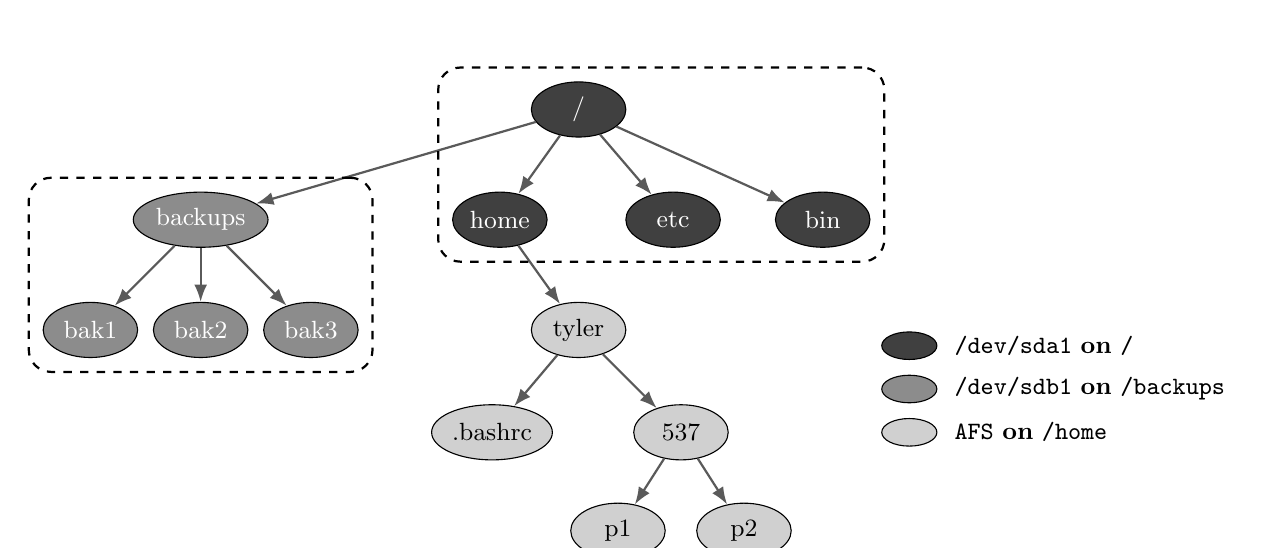
\begin{tikzpicture}[>={Latex[length=2.2mm]},
    fsA/.style={ellipse, draw, fill=black!75, text=white, minimum width=1.2cm, minimum height=0.7cm, inner sep=1pt, font=\small},
    fsB/.style={ellipse, draw, fill=black!45, text=white, minimum width=1.2cm, minimum height=0.7cm, inner sep=1pt, font=\small},
    fsC/.style={ellipse, draw, fill=g1, text=black, minimum width=1.2cm, minimum height=0.7cm, inner sep=1pt, font=\small}]
  \node[fsA] (r) at (6.2,0) {/};
  \node[fsB] (bk) at (1.4,-1.4) {backups};
  \node[fsA] (hm) at (5.2,-1.4) {home};
  \node[fsA] (etc) at (7.4,-1.4) {etc};
  \node[fsA] (bin) at (9.3,-1.4) {bin};
  \node[fsB] (b1) at (0,-2.8) {bak1};
  \node[fsB] (b2) at (1.4,-2.8) {bak2};
  \node[fsB] (b3) at (2.8,-2.8) {bak3};
  \node[fsC] (ty) at (6.2,-2.8) {tyler};
  \node[fsC] (bash) at (5.1,-4.1) {.bashrc};
  \node[fsC] (c5) at (7.5,-4.1) {537};
  \node[fsC] (p1) at (6.7,-5.35) {p1};
  \node[fsC] (p2) at (8.3,-5.35) {p2};
  \foreach \a/\b in {r/bk, r/hm, r/etc, r/bin, bk/b1, bk/b2, bk/b3, hm/ty, ty/bash, ty/c5, c5/p1, c5/p2}
    \draw[->, thick, g3] (\a) -- (\b);
  \node[draw, dashed, thick, rounded corners=8pt, inner sep=5pt, fit=(r)(hm)(etc)(bin)] {};
  \node[draw, dashed, thick, rounded corners=8pt, inner sep=5pt, fit=(bk)(b1)(b2)(b3)] {};
  % legend
  \node[fsA, minimum width=0.7cm, minimum height=0.35cm] at (10.4,-3.0) {};
  \node[anchor=west, font=\small] at (10.85,-3.0) {\texttt{/dev/sda1} \textbf{on} \texttt{/}};
  \node[fsB, minimum width=0.7cm, minimum height=0.35cm] at (10.4,-3.55) {};
  \node[anchor=west, font=\small] at (10.85,-3.55) {\texttt{/dev/sdb1} \textbf{on} \texttt{/backups}};
  \node[fsC, minimum width=0.7cm, minimum height=0.35cm] at (10.4,-4.1) {};
  \node[anchor=west, font=\small] at (10.85,-4.1) {\texttt{AFS} \textbf{on} \texttt{/home}};
\end{tikzpicture}
\end{center}
{\small (The slide uses green, red and blue for the three file systems; here
they are dark, medium and light grey.)}
\keepspace{0pt}

Lookups simply continue into the mounted file system at a mount point, so
paths alone are enough.

\keepspace{7\baselineskip}
% ===========================================================================
\section{Summary}
% ===========================================================================

\begin{keybox}[File system API]
\begin{itemize}
  \item Using \textbf{multiple types of name} provides
        \textbf{convenience} (paths) and \textbf{efficiency} (inode numbers,
        file descriptors: traverse once).
  \item \textbf{Mount} and \textbf{link} features provide
        \textbf{flexibility}.
  \item \textbf{Special calls} (\texttt{fsync}, \texttt{rename}) let
        developers communicate special requirements to the file system.
\end{itemize}
\end{keybox}

\begin{center}
\small
\renewcommand{\arraystretch}{1.15}
\begin{tabularx}{\textwidth}{@{}lX@{}}
  \toprule
  \textbf{Call} & \textbf{What it does} \\
  \midrule
  \texttt{open(path, flags, mode)} & traverse the path once, create an open file object (offset 0), return the lowest free fd \\
  \texttt{read(fd, buf, n)} & read up to \(n\) bytes at the current offset; returns bytes read (0 at end of file); offset \(+=\) bytes read \\
  \texttt{write(fd, buf, n)} & write up to \(n\) bytes at the current offset (buffered in memory); returns the number actually written (may be fewer) \\
  \texttt{close(fd)} & free the fd slot; open file object freed when no fd refers to it \\
  \texttt{dup(fd)} & new fd sharing the same open file object (same offset) \\
  \texttt{lseek(fd, off, whence)} & set the offset (\texttt{SEEK\_SET}, \texttt{SEEK\_CUR}, \texttt{SEEK\_END}); no disk I/O \\
  \texttt{fsync(fd)} & force the file's dirty data and its metadata (inode, size) to disk; returns when done (sometimes also needed on the directory) \\
  \texttt{rename(old, new)} & change a file's name atomically (used by \texttt{mv} and for atomic file updates) \\
  \texttt{stat(path)}, \texttt{fstat(fd)} & fill a \texttt{struct stat} with the inode's metadata (size, inode number, links, owner, times, \ldots) \\
  \texttt{unlink(path)} & remove a name, decrement the link count; free inode and data at 0 (used by \texttt{rm}) \\
  \texttt{mkdir(path, mode)} & create an empty directory (only \texttt{.} and \texttt{..}) \\
  \texttt{opendir}, \texttt{readdir}, \texttt{closedir} & read a directory one \texttt{struct dirent} (name, inode number, \ldots) at a time \\
  \texttt{rmdir(path)} & delete a directory; fails unless it is empty \\
  \texttt{link(old, new)} & hard link: a new name for the same inode (\texttt{ln}) \\
  \texttt{symlink} (via \texttt{ln -s}) & symbolic link: a new file whose data is the target's pathname \\
  \texttt{mount} & attach a file system at a directory of the single tree \\
  \bottomrule
\end{tabularx}
\end{center}

\end{document}
